\documentclass[compress]{beamer}

%PACKAGE
%----------------------------------
\usepackage{graphicx}
\graphicspath{{Images/}}

\usepackage{xcolor}
\newcommand{\rc}[1]{{\color{red}{#1}}}
\newcommand{\bc}[1]{{\color{blue}{#1}}}

\usepackage{amsmath, amssymb}
\usepackage{bm, bbm}
\usepackage{caption, subcaption}
\usepackage{bibentry, natbib}
\usepackage{appendix}
\usepackage{outlines}
\usepackage{setspace}
\usepackage{comment}
\usepackage{multicol, multirow, array}
\usepackage{tabu}
\usepackage{algorithm2e, algorithmic}
\usepackage{float}
\usepackage{array}
\usepackage{booktabs}
\usepackage[flushleft]{threeparttable}
\usepackage{tikz}

\usepackage{hyperref}
\hypersetup{
	colorlinks=true,
	linkcolor=blue,
	filecolor=blue,      
	urlcolor=blue,
	citecolor=black
}

% --- notation macros ---
\newcommand{\PP}{\mathbb{P}}
\newcommand{\QQ}{\mathbb{Q}}
\newcommand{\EE}{\mathbb{E}}
\newcommand{\FF}{\mathcal{F}}
\newcommand{\dd}{\,\mathrm{d}}

\newcommand\MyBox[2]{
	\fbox{\lower0.75cm
		\vbox to 1.7cm{\vfil
			\hbox to 1.7cm{\hfil\parbox{1.4cm}{#1\\#2}\hfil}
			\vfil}%
	}%
}

\usetheme{Frankfurt}
\usecolortheme{seahorse}
\setbeamertemplate{footline}[frame number]
\setbeamertemplate{navigation symbols}{}
\AtBeginSection[]{
	\begin{frame}
		\vfill
		\centering
		\begin{beamercolorbox}[sep=8pt,center,shadow=true,rounded=true]{title}
			\usebeamerfont{title}\insertsectionhead\par%
		\end{beamercolorbox}
		\vfill
	\end{frame}
}

%TITLE
%-----
\title[CIR \& Bond Pricing]{Short-Rate Models and Bond Pricing}
\author[\textbf{Auteur}]{\textbf{Auteur}}
\date{\today}


\AtBeginSubsection[]
{
	\begin{frame}<beamer>{Outline}
		\tableofcontents[currentsection,currentsubsection]
	\end{frame}
}

%----------------------------------------------------------------
\begin{document}
\bibliographystyle{apalike}

\begin{frame}
	\titlepage
\end{frame}

{\AtBeginSection{}}

%============================================================
\section{Spot Rate, Forward Rates, and the Zero-Coupon Yield Curve}
%============================================================

%--- Slide 1 --------------------------------------------------
\begin{frame}{The Zero-Coupon Bond: The Fundamental Building Block}

\textbf{Definition.} A \textit{zero-coupon bond} with maturity $T$ pays \$1 at time $T$ and nothing before.
\[
	P(t,T) \;=\; \text{price at time } t \le T.
\]

\medskip
\textbf{Risk-neutral pricing formula:}
\[
	\boxed{P(t,T) \;=\; \EE^{\QQ}\!\left[\,e^{-\int_t^T r_s\,\dd s}\;\Big|\;\FF_t\right]}
\]

\medskip
\begin{itemize}
	\item $e^{-\int_t^T r_s\,\dd s}$: stochastic discount factor from $t$ to $T$.
	\item $r_s$: the \textit{instantaneous short rate} at time $s$.
	\item $P(t,t) = 1$ (a bond that matures now is worth its face value).
	\item $P(t,T) \in (0,1]$ under positive interest rates.
\end{itemize}

\end{frame}

%--- Slide 2 --------------------------------------------------
\begin{frame}{Where Does This Formula Come From?}

\textbf{Start in discrete time.}  In a one-period world with constant rate $r$, the discounted price process is:
\[
	B_t^{-1} \cdot S_t \;=\; S_t \cdot \prod_{k} \frac{1}{1+r\,\Delta t}.
\]

\medskip
\textbf{Pass to continuous time.}  With a \textit{constant} continuously-compounded rate $r$, the money-market account is $B_t = e^{rt}$, so:
\[
	B_t^{-1} S_t \;=\; S_t\,e^{-rT}.
\]

\medskip
\textbf{Problem.}  A single constant rate over the whole period is unrealistic:
\begin{itemize}
	\item The economy faces different inflation pressures over time.
	\item The time-value of money is constantly changing.
	\item $\Rightarrow$ We need to \textit{generalize} the discounted price process.
\end{itemize}

\end{frame}

%--- Slide 3 --------------------------------------------------
\begin{frame}{The Instantaneous Short Rate and Money-Market Account}

\textbf{Key idea.}  Let the interval $[0,T]$ be sliced into infinitesimally small pieces of length $\Delta t \to 0$. In each piece $[t, t+\Delta t]$, the rate is $r_t$.

\medskip
Letting $\Delta t \to 0$, we obtain a \textit{single rate for an infinitesimally short period}: the \textbf{instantaneous short rate} $r_t$.

\medskip
\textbf{The money-market account.}  Investing \$1 at time 0 and continuously rolling over at $r_t$:
\[
	B_t \;=\; \exp\!\left(\int_0^t r_s\,\dd s\right), \qquad \frac{\dd B_t}{B_t} = r_t\,\dd t.
\]

\medskip
\textbf{The discounted price process} is now generalized to constantly changing rates:
\[
	B_t^{-1} S_t \;=\; S_t \cdot \exp\!\left(-\int_0^t r_s\,\dd s\right).
\]

\end{frame}

%--- Slide 4 --------------------------------------------------
\begin{frame}{Bond Yield and the Yield Curve}

\textbf{Bond price from yield.}  We write the zero-coupon bond price as:
\[
	P(t,T) \;=\; e^{-y(t,T)\,(T-t)},
\]
where $y(t,T)$ is the \textbf{continuously-compounded zero-coupon yield}.

\medskip
\textbf{Solving for the yield:}
\[
	y(t,T) \;=\; -\frac{1}{T-t}\,\ln P(t,T).
\]

\medskip
$y(t,T)$ is the constant rate that would give the \textit{same} bond price as the full stochastic discounting — a summary statistic of the bond.

\medskip
\textbf{Since bonds have many maturities} ($T = 1, 2, 5, 30, \ldots$ years), the function $T \mapsto y(t,T)$ traces the \textbf{zero-coupon yield curve} at time $t$.

\medskip
\begin{center}
\small
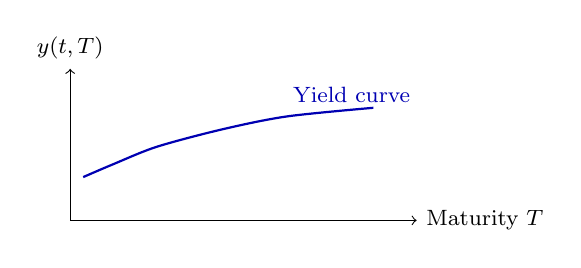
\begin{tikzpicture}[scale=0.55]
  \draw[->](0,0)--(8,0) node[right]{\footnotesize Maturity $T$};
  \draw[->](0,0)--(0,3.5) node[above]{\footnotesize $y(t,T)$};
  \draw[thick,blue!70!black] plot[smooth] coordinates
    {(0.3,1.0)(1,1.3)(2,1.7)(3.5,2.1)(5,2.4)(7,2.6)};
  \node[blue!70!black,font=\footnotesize] at (6.5,2.9) {Yield curve};
\end{tikzpicture}
\end{center}

\end{frame}

%--- Slide 5 --------------------------------------------------
\begin{frame}{Forward Rates: The Marginal Rate at a Future Date}

\textbf{The instantaneous forward rate} $f(t,T)$ is the marginal rate the market implies for borrowing over an infinitesimally short interval around a \textit{future} date $T$, as seen from time $t$:
\[
	f(t,T) \;:=\; -\frac{\partial}{\partial T}\ln P(t,T).
\]

\medskip
\textbf{Intuition.}  $f(t,T)\,\Delta T$ $\approx$ rate paid (locked in today at $t$) for borrowing from $T$ to $T+\Delta T$.

\medskip
\textbf{Bootstrapping forward rates from bond prices.}
Integrating $f(t,T) = -\partial_T \ln P(t,T)$ over $[t,T]$ and using $P(t,t) = 1$:
\[
	\boxed{P(t,T) \;=\; \exp\!\left(-\int_t^T f(t,u)\,\dd u\right).}
\]
Bond price = exponential of the \textit{area under the forward curve} from $t$ to $T$.

\medskip
\textbf{Yield as average of forward rates:}
\[
	y(t,T) \;=\; \frac{1}{T-t}\int_t^T f(t,u)\,\dd u.
\]

\end{frame}

%--- Slide 6 --------------------------------------------------
\begin{frame}{The Yield Curve and Forward Curve Together}

\begin{center}
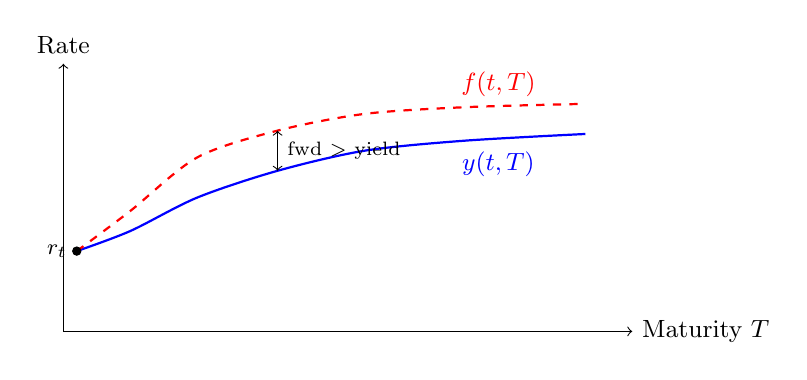
\begin{tikzpicture}[scale=0.85]
  \draw[->](0,0)--(8.5,0) node[right]{\small Maturity $T$};
  \draw[->](0,0)--(0,4.0) node[above]{\small Rate};
  \draw[thick,blue] plot[smooth] coordinates
    {(0.2,1.2)(1.0,1.5)(2.0,2.0)(3.2,2.4)(4.5,2.7)(6.0,2.85)(7.8,2.95)};
  \draw[thick,red,dashed] plot[smooth] coordinates
    {(0.2,1.2)(1.0,1.8)(2.0,2.6)(3.2,3.0)(4.5,3.25)(6.0,3.35)(7.8,3.4)};
  \fill[black](0.2,1.2) circle (2pt) node[left]{\footnotesize $r_t$};
  \node[blue] at (6.5,2.5) {\small $y(t,T)$};
  \node[red] at (6.5,3.7) {\small $f(t,T)$};
  \draw[<->](3.2,2.4)--(3.2,3.0) node[midway,right,font=\scriptsize]{fwd $>$ yield};
\end{tikzpicture}
\end{center}

\medskip
Key facts:
\begin{itemize}
	\item Both curves pass through $r_t$ as $T \to t$ (the short rate).
	\item $f(t,T) > y(t,T)$ when the yield curve is upward-sloping.
	\item $r_t = \lim_{T\downarrow t} y(t,T) = f(t,t)$: the short rate is the \textit{instantaneous} yield.
\end{itemize}

\end{frame}

%--- Slide 7 --------------------------------------------------
\begin{frame}{The Key Relationship: Discount Rates and Forward Rates}

\textbf{Under $\QQ$}, combining the two representations:

\medskip
\begin{columns}
\column{0.48\textwidth}
\textbf{Discounted price process}
\[
	B_t^{-1} S_t = S_t\,e^{-\int_0^t r_s\,\dd s}
\]
(\textcolor{blue}{known up to time $t$})

\column{0.48\textwidth}
\textbf{Bond price}
\[
	P(t,T) = e^{-\int_t^T f(t,u)\,\dd u}
\]
(\textcolor{red}{instantaneous forward rates})
\end{columns}

\medskip\medskip
We establish the fundamental relationship:
\[
	P(t,T)
	\;=\; \EE^{\QQ}\!\!\left[e^{-\int_t^T r_s\,\dd s}\,\Big|\,\FF_t\right]
	\;=\; e^{-\int_t^T f(t,u)\,\dd u}.
\]

\medskip
Differentiating with respect to $T$:
\[
	f(t,T) \;=\; -\frac{\partial}{\partial T}\ln P(t,T).
\]

This allows \textit{bootstrapping} $f(t,T)$ from market bond prices at time $t$.

\end{frame}

%--- Slide 8 --------------------------------------------------
\begin{frame}{Why Do We Need to Model $r_t$?}

In a simple market model with \textit{constant} rates, discounting is trivial. But:

\medskip
\begin{itemize}
	\item The economy is always subject to different rates and inflationary pressures.
	\item The time-value of money is \textit{constantly changing}.
\end{itemize}

\medskip
\textbf{Advantages of the instantaneous short rate $r_t$:}
\begin{itemize}
	\item Flexible — accounts for a changing interest rate environment.
	\item Allows exact discounting at each instant.
\end{itemize}

\medskip
\textbf{New problem this creates:}
\begin{itemize}
	\item The risk from rates is now something we need to \textit{model and predict} to ensure fair, no-arbitrage pricing.
	\item Under $\PP$: $r_t$ follows dynamics calibrated to historical data.
	\item Under $\QQ$: $r_t$ follows risk-neutral dynamics used for pricing.
\end{itemize}

$\Rightarrow$ We need a stochastic model for $r_t$ and a way to change measure.

\end{frame}

%============================================================
\section{Risk-Neutral Dynamics Under $\QQ$: The CIR Model}
%============================================================

%--- Slide 9 --------------------------------------------------
\begin{frame}{CIR Under the Physical Measure $\PP$}

\textbf{Assumption:} We work on $(\Omega, \FF, (\FF_t)_{t\ge 0}, \PP)$.

\medskip
The \textbf{Cox--Ingersoll--Ross (CIR)} model specifies the short rate under $\PP$:
\[
	\dd r_t \;=\; \kappa_\PP\!\left(\theta_\PP - r_t\right)\dd t \;+\; \sigma\sqrt{r_t}\,\dd W_t^\PP,
	\qquad r_0 > 0.
\]

\medskip
\begin{itemize}
	\item $\kappa_\PP > 0$: speed of mean reversion.
	\item $\theta_\PP > 0$: long-run level under $\PP$ (physical equilibrium rate).
	\item $\sigma > 0$: volatility parameter.
	\item $\sigma\sqrt{r_t}$: \textit{state-dependent} volatility — higher when rates are higher.
\end{itemize}

\medskip
\textbf{Feller condition} (for strict positivity):
\[
	2\kappa_\PP\theta_\PP \;\ge\; \sigma^2
	\quad \Rightarrow \quad r_t > 0 \;\text{ a.s.\ for all } t.
\]

\end{frame}

%--- Slide 10 --------------------------------------------------
\begin{frame}{Why Can't We Price Directly Under $\PP$?}

\textbf{No-arbitrage requires a risk-neutral measure $\QQ$.}

\medskip
\begin{itemize}
	\item Under $\PP$: expectations reflect \textit{real-world} probabilities.
	\item For pricing: we need $\QQ$ under which every discounted asset is a \textit{martingale}.
	\item $\PP$ and $\QQ$ are \textbf{equivalent} (agree on zero-probability events) but assign different probabilities to non-null events.
\end{itemize}

\medskip
\textbf{Radon-Nikodym derivative} (the ``exchange rate'' between measures):
\[
	\EE^{\QQ}[X] \;=\; \EE^{\PP}\!\!\left[X\cdot\frac{\dd\QQ}{\dd\PP}\right].
\]

\medskip
The bridge between $\PP$ and $\QQ$ for Brownian-driven models is \textbf{Girsanov's theorem}.

\end{frame}

%--- Slide 11 --------------------------------------------------
\begin{frame}{Girsanov's Theorem}

\textbf{Setup.}  Let $(\lambda_t)_{t\ge 0}$ be an adapted process (the \textit{market price of risk}). Define:
\[
	Z_T \;=\; \exp\!\left(-\int_0^T \lambda_s\,\dd W_s^\PP \;-\; \frac{1}{2}\int_0^T \lambda_s^2\,\dd s\right).
\]

Set $\dfrac{\dd\QQ}{\dd\PP}\Big|_{\FF_T} = Z_T$.

\medskip
\textbf{Girsanov's theorem:}  Under $\QQ$, the process
\[
	W_t^\QQ \;:=\; W_t^\PP + \int_0^t \lambda_s\,\dd s
\]
is a \textbf{standard Brownian motion}.

\medskip
\textbf{Equivalently:} $\dd W_t^\PP = \dd W_t^\QQ - \lambda_t\,\dd t$.

\medskip
\textbf{Intuition.} We add a deterministic drift $\lambda_t\,\dd t$ to the $\PP$-Brownian motion. The ``new'' randomness is now centred under $\QQ$.

\end{frame}

%--- Slide 12 --------------------------------------------------
\begin{frame}{From $\PP$ to $\QQ$: Rewriting the CIR SDE}

\textbf{Under $\PP$:}
\[
	\dd r_t = \kappa_\PP(\theta_\PP - r_t)\,\dd t + \sigma\sqrt{r_t}\,\dd W_t^\PP.
\]

Substituting $\dd W_t^\PP = \dd W_t^\QQ - \lambda_t\,\dd t$:
\[
	\dd r_t
	= \underbrace{\kappa_\PP(\theta_\PP - r_t)\,\dd t}_{\text{physical drift}}
	+ \sigma\sqrt{r_t}\!\underbrace{(\dd W_t^\QQ - \lambda_t\,\dd t)}_{\dd W_t^\PP}
\]

\medskip
Expanding:
\[
	\dd r_t
	= \Big[\kappa_\PP(\theta_\PP - r_t) - \sigma\sqrt{r_t}\,\lambda_t\Big]\dd t
	+ \sigma\sqrt{r_t}\,\dd W_t^\QQ.
\]

\medskip
\textbf{Goal:} choose $\lambda_t$ so that the $\QQ$-drift is again \textit{affine in $r_t$}:
\[
	\dd r_t = \kappa_\QQ(\theta_\QQ - r_t)\,\dd t + \sigma\sqrt{r_t}\,\dd W_t^\QQ.
\]

Note: Girsanov changes only the \textit{drift} — the diffusion coefficient $\sigma\sqrt{r_t}$ is \textbf{the same under both measures}.

\end{frame}

%--- Slide 13 --------------------------------------------------
\begin{frame}{The Required Form of $\lambda_t$}

\textbf{Matching the drift.}  We need:
\[
	\kappa_\PP(\theta_\PP - r_t) - \sigma\sqrt{r_t}\,\lambda_t
	\;=\; \kappa_\QQ\theta_\QQ - \kappa_\QQ r_t.
\]

\medskip
For this to hold for all $r_t > 0$ with the CIR structure preserved, set:
\[
	\lambda_t \;=\; \eta\sqrt{r_t}, \qquad \eta \in \mathbb{R}.
\]

\medskip
This gives the \textbf{risk-neutral parameters}:
\[
	\boxed{
	\kappa_\QQ \;=\; \kappa_\PP + \sigma\eta,
	\qquad
	\kappa_\QQ\theta_\QQ \;=\; \kappa_\PP\theta_\PP.
	}
\]

\medskip
\begin{itemize}
	\item $\lambda_t = \eta\sqrt{r_t}$: risk premium is proportional to $\sqrt{r_t}$ — higher when rates are high.
	\item $\kappa_\QQ\theta_\QQ = \kappa_\PP\theta_\PP$: product of speed and long-run level is \textit{preserved} under the measure change.
	\item Diffusion coefficient $\sigma\sqrt{r_t}$ is unchanged under $\QQ$.
\end{itemize}

\end{frame}

%--- Slide 14 --------------------------------------------------
\begin{frame}{The Feller Condition: Keeping Rates Positive}

\textbf{CIR under $\QQ$:}
\[
	\dd r_t = \kappa_\QQ(\theta_\QQ - r_t)\,\dd t + \sigma\sqrt{r_t}\,\dd W_t^\QQ.
\]

\medskip
\textbf{Behavior near $r_t = 0$:}
\begin{itemize}
	\item Diffusion $\sigma\sqrt{r_t} \approx 0$: very little noise.
	\item Drift $\kappa_\QQ\theta_\QQ > 0$: pushes rate \textit{upward}.
	\item When $r_t < \theta_\QQ$: upward pull; when $r_t > \theta_\QQ$: downward pull.
\end{itemize}

\medskip
\textbf{Feller condition:}
\[
	2\kappa_\QQ\theta_\QQ \;\ge\; \sigma^2.
\]
Guarantees: upward drift at zero is strong enough to prevent $r_t$ from reaching 0.

\medskip
\begin{tabular}{lll}
\toprule
$2\kappa\theta > \sigma^2$ & Strict Feller & $r_t > 0$ a.s.\ (zero \textit{inaccessible}) \\
$2\kappa\theta = \sigma^2$ & Boundary & $r_t$ touches 0 but reflects instantly \\
$2\kappa\theta < \sigma^2$ & Violated & $r_t$ can spend time at 0 \\
\bottomrule
\end{tabular}

\medskip
\small Note: violating Feller does \textbf{not} destroy the strong solution — $r_t \ge 0$ a.s.\ in all cases.

\end{frame}

%--- Slide 15 --------------------------------------------------
\begin{frame}{The Novikov Condition}

\textbf{Why we need it.}  For $Z_T = \exp\!\big(-\int_0^T \lambda_s\,\dd W_s^\PP - \frac{1}{2}\int_0^T \lambda_s^2\,\dd s\big)$ to define a valid probability measure $\QQ$, $Z_T$ must be a \textit{true martingale} (not merely local).

\medskip
\textbf{Novikov condition} (sufficient):
\[
	\EE^{\PP}\!\left[\exp\!\left(\frac{1}{2}\int_0^T \lambda_t^2\,\dd t\right)\right] < \infty.
\]

\medskip
\textbf{Verification for $\lambda_t = \eta\sqrt{r_t}$.}
\[
	\frac{1}{2}\int_0^T \lambda_t^2\,\dd t \;=\; \frac{\eta^2}{2}\int_0^T r_t\,\dd t.
\]
We need: $\;\EE^{\PP}\!\big[\exp\!\big(\tfrac{\eta^2}{2}\int_0^T r_t\,\dd t\big)\big] < \infty$.

\medskip
Since CIR is an \textbf{affine process}, its moment generating function for $\int_0^T r_t\,\dd t$ is exponential-affine in $r_0$ and \textit{finite on any finite horizon $T$}.

\medskip
$\Rightarrow$ \textbf{Novikov condition is satisfied} for any finite $T$ and any $\eta \in \mathbb{R}$.

\end{frame}

%--- Slide 16 --------------------------------------------------
\begin{frame}{Why $\lambda_t = \eta\sqrt{r_t}$ Is the Natural Choice}

\textbf{The problem with other choices of $\lambda_t$.}

\medskip
Suppose instead $\lambda_t = \zeta / \sqrt{r_t}$ (e.g.\ if we tried a constant-volatility correction):
\begin{itemize}
	\item As $r_t \to 0$: $\lambda_t \to \infty$ — the integrand blows up.
	\item $\int_0^T \lambda_t^2\,\dd t = \zeta^2\int_0^T r_t^{-1}\,\dd t$ can be \textbf{unbounded}.
	\item Novikov condition \textit{may fail} — $\QQ$ would not be a valid probability measure.
\end{itemize}

\medskip
\textbf{Why $\lambda_t = \eta\sqrt{r_t}$ works:}
\begin{itemize}
	\item As $r_t \to 0$: $\lambda_t \to 0$ — the market price of risk vanishes.
	\item $\int_0^T \eta^2 r_t\,\dd t$ is bounded (CIR is mean-reverting and non-negative).
	\item Novikov condition holds on any finite $[0,T]$.
	\item \textit{CIR structure is preserved} under $\QQ$.
\end{itemize}

\medskip
\textbf{Economic interpretation:} risk compensation $\propto \sqrt{r_t}$ — higher when rates are elevated, near zero in a liquidity-trap environment.

\end{frame}

%--- Slide 17 --------------------------------------------------
\begin{frame}{CIR Preserved Under $\QQ$: Full Derivation}

Starting from the $\PP$-dynamics and substituting $\dd W_t^\PP = \dd W_t^\QQ - \eta\sqrt{r_t}\,\dd t$:

\begin{align*}
	\dd r_t
	&= \Big[\kappa_\PP(\theta_\PP - r_t) - \sigma\sqrt{r_t} \cdot \eta\sqrt{r_t}\Big]\dd t + \sigma\sqrt{r_t}\,\dd W_t^\QQ \\
	&= \Big[\kappa_\PP\theta_\PP - \kappa_\PP r_t - \sigma\eta r_t\Big]\dd t + \sigma\sqrt{r_t}\,\dd W_t^\QQ \\
	&= \Big[\kappa_\PP\theta_\PP - (\kappa_\PP + \sigma\eta)\,r_t\Big]\dd t + \sigma\sqrt{r_t}\,\dd W_t^\QQ.
\end{align*}

Set $\kappa_\QQ := \kappa_\PP + \sigma\eta$ and $\theta_\QQ := \dfrac{\kappa_\PP\theta_\PP}{\kappa_\QQ}$. Then:

\[
	\boxed{\dd r_t \;=\; \kappa_\QQ(\theta_\QQ - r_t)\,\dd t + \sigma\sqrt{r_t}\,\dd W_t^\QQ.}
\]

\medskip
The \textbf{CIR structure is fully preserved} under $\QQ$:
\begin{itemize}
	\item Same diffusion coefficient $\sigma\sqrt{r_t}$ (Girsanov only changes the drift).
	\item Same affine structure $\Rightarrow$ closed-form bond pricing formulas.
	\item Feller condition: $2\kappa_\QQ\theta_\QQ = 2\kappa_\PP\theta_\PP \ge \sigma^2$ — \textit{automatically inherited}.
\end{itemize}

\end{frame}

%--- Slide 18 --------------------------------------------------
\begin{frame}{Summary: $\PP$--$\QQ$ Relationship in the CIR Model}

\begin{center}
\renewcommand{\arraystretch}{1.4}
\begin{tabular}{lcc}
\toprule
& Under $\PP$ & Under $\QQ$ \\
\midrule
SDE & $\kappa_\PP(\theta_\PP - r_t)\,\dd t + \sigma\sqrt{r_t}\,\dd W_t^\PP$ 
    & $\kappa_\QQ(\theta_\QQ - r_t)\,\dd t + \sigma\sqrt{r_t}\,\dd W_t^\QQ$ \\
Speed & $\kappa_\PP$ & $\kappa_\QQ = \kappa_\PP + \sigma\eta$ \\
Long-run & $\theta_\PP$ & $\theta_\QQ = \kappa_\PP\theta_\PP / \kappa_\QQ$ \\
Diffusion & $\sigma\sqrt{r_t}$ & $\sigma\sqrt{r_t}$ (unchanged) \\
\bottomrule
\end{tabular}
\end{center}

\medskip
\textbf{Key invariants:}
\[
	\kappa_\QQ\theta_\QQ \;=\; \kappa_\PP\theta_\PP \qquad (\text{Feller constant preserved})
\]
\[
	\sigma \;\text{ is the same under both measures.}
\]

\medskip
\textbf{Next:} Use the $\QQ$-dynamics to show the discounted bond price is a $\QQ$-martingale, then derive the log-affine CIR bond pricing formula via Feynman-Kac.

\end{frame}

\appendix

\begin{comment}
\end{comment}

\end{document}
